\subsection{Energy Harvesting Systems}
\label{sec:background_harvesting}

Energy harvesting devices operate using energy extracted from ambient sources, e.g., radio frequency transmissions, light, etc. These devices elide tethered power and batteries, instead collecting energy into a capacitor, operating when sufficient charge accumulates, and turning off for recharge upon depletion of the buffer. There are several energy harvesting battery-less platforms. For instance, computational RFIDs---open-source TI MSP430-based~\cite{wolverine} WISP~\cite{wisp5} (with its variants such as WISPCam~\cite{naderiparizi_rfid_2015}, NFC-WISP~\cite{zhao_rfid_2015} or NeuralWISP~\cite{holleman_biocas_2008}), Moo~\cite{moo}, and commercial ones such as~\cite{medusa_farsens_2017}. Other platforms include ambient backscatter tag~\cite{liu_sigcomm_2013,parks_sigcomm_2014} or battery-less phone~\cite{talla_imwut_2017}. 
%
% \textbf{Target Hardware of \sys.}
\sys is designed for the demands of existing and future \emph{tiny embedded energy-harvesting platforms} based around general purpose, commodity computing components~\cite{wisp,msp430datasheet}. \sys targets a device with a memory system that has fast, byte-addressable volatile and non-volatile memory; in particular, our target platform, WISP~\cite{wisp}, is equipped with a mixture of SRAM and FRAM. \sys leverages hardware support for fast, bulk-copying between memories via DMA~\cite{msp430datasheet}. \sys does not require architectural additions to commodity processors as in~\cite{su_date_2017,hicks_isca_2017,quickrecall,nvp}.

\subsection{Intermittent Execution}
\label{sec:background_consistency}

% Table
\begin{table}%
\caption{Simulation Configuration}
\label{tab:one}
\begin{minipage}{\columnwidth}
\begin{center}
\begin{tabular}{ll}
  \toprule
        Model & Data Copied to/from NVRAM \\
        \hline
        Mementos~\cite{mementos}    & Registers + Stack     \\
        DINO~\cite{dino}    & Registers + Stack + WAR NV variables \\%used in task\\
        Chain~\cite{chain}  & PC + NV variables used in task\\
        Alpaca~\cite{alpaca}    & PC + WAR NV variables used in task\\
        Ratchet~\cite{ratchet}, Clank~\cite{hicks_isca_2017} & Registers (requires NV main memory) \\
        Region Formation~\cite{baghsorkhi_cgo_2018} & Registers + Updated variables in task \\
  \bottomrule
\end{tabular}
\end{center}
\end{minipage}
  \label{table:chechpoint_comparison}
\end{table}%

%\begin{table}
%    \centering
%    \begin{tabular}{|c|c|}
%        \hline
%        Model & Data Copied to/from NVRAM \\
%        \hline
%        Mementos~\cite{mementos}    & Registers + Stack     \\
%        DINO~\cite{dino}    & Registers + Stack + WAR NV variables \\%used in task\\
%        Chain~\cite{chain}  & PC + NV variables used in task\\
%        Alpaca~\cite{alpaca}    & PC + WAR NV variables used in task\\
%        Ratchet~\cite{ratchet}, Clank~\cite{hicks_isca_2017} & Registers (requires NV main memory) \\
%        Region Formation~\cite{baghsorkhi_cgo_2018} & Registers + Updated variables in task \\
%        \hline
%    \end{tabular}
%    \caption{Non-volatile memory access for data consistency; {PC}: program counter, {WAR variables}: variables involved in Write-after-Read (WAR) dependencies, {NV}: non-volatile.}
%    \label{table:chechpoint_comparison}
%\end{table}

Software running on an energy-harvesting device executes {\em intermittently} because power sources are not always available to harvest and buffer sufficient operational energy. An intermittent execution is composed of operating periods interspersed with power failures~\cite{dino,chain,alpaca,ratchet}. The frequency of failures depends on the size of the device's energy storage buffer (a larger buffer allows longer operating periods), current consumption and incoming energy.

\begin{figure}		
	\centering
	\begin{minipage}{.8\textwidth}
	\begin{subfigure}{.5\columnwidth}
			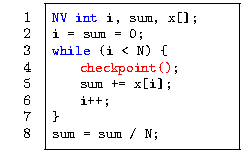
\includegraphics[width=\columnwidth, trim={.3cm 0 0 0}]{figures/war-example.pdf}
		\caption{WAR-affected code}
		\label{fig:war-example}
	\end{subfigure}
	\begin{subfigure}{.5\columnwidth}
			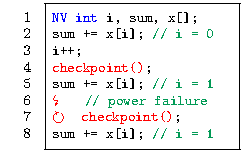
\includegraphics[width=\columnwidth,trim={.3cm 0 0 0 }  ]{figures/war-execution.pdf}
		\caption{WAR-affected execution}
		\label{fig:war-execution}
	\end{subfigure}
	\caption{WAR dependency example. \texttt{NV} marks non-volatile variables, \texttt{checkpoint()} is a checkpoint of volatile state.	\label{fig:w-a-r}}
	\end{minipage}
\end{figure}

A power failure clears volatile state (e.g., registers and SRAM) while non-volatile memory (e.g., FRAM) persists. Upon a power failure, control flows to a prior point in the execution: by default, to the beginning of {\tt main()}. Early intermittent systems preserved progress by periodically checkpointing volatile execution context to non-volatile memory~\cite{mementos}, sometimes requiring hardware support~\cite{mottola2017harvos,hibernusplusplus,hibernus,idetic,quickrecall}, Table~\ref{table:chechpoint_comparison} summarizes the data that gets copied to and from the non-volatile memory in service of memory consistency and progress preservation. Checkpointing volatile state alone does not ensure data consistency when the system can directly manipulate non-volatile memory~\cite{mspcdino}. Precisely, data can get inconsistent when code includes a \emph{write-after-read} (WAR) dependency between operations that manipulate non-volatile memory. Fig.~\ref{fig:w-a-r} illustrates how state can become inconsistent in an intermittent execution using a simple example of an average operation over an array of integers.
The non-volatile variable \texttt{sum} introduces the WAR, being read and written sequentially by the increment operation. If a power failure occurs right before updating the non-volatile index \texttt{i} (Fig.~\ref{fig:war-execution}, Line 6), \texttt{sum} gets erroneously incremented twice consecutively by the same array element (Fig.~\ref{fig:war-execution}, Lines 5 and 8).

\subsection{Task-based Intermittent Programming}
\label{section:background_task_computing}

Task-based execution models~\cite{dino,chain,alpaca} ask the programmer to decompose their program into \textbf{tasks}, which are regions of code that can contain arbitrary computation, sensing, and communication. Task-based models progress at the granularity of tasks. They re-execute each task interrupted by a power failure until it successfully finishes, only then moving on to the next task. Since these models do not rely on capturing an expensive checkpoint, they are usually faster than the checkpoint-based solution~\cite{chain, alpaca}.  \sys also follows the paradigm of the task-based programming model, where the programmer explicitly expresses the application as a sequence of tasks and the transitions between them.

Task-based models also suffer from data inconsistencies when WAR dependencies are involved. Prior systems tried to tackle this problem by a compiler-automated redo-logging for the variables that are part of the dependency~\cite{alpaca}, or by statically creating multiple copies of the problematic variable to ensure that no task reads and writes the same copy~\cite{chain}.

\subsection{Costs of Previous Models}
\label{sec:cost_task-based}

Prior systems, including task-based models, have two major drawbacks: {\em frequent non-volatile memory accesses} and {\em incorrectly sized tasks} (too small or too large).

%\textbf{Direct Non-volatile Memory Access.} Previous systems frequently access the non-volatile memory directly, which is a potential source of inefficiency. Checkpointing systems copy all volatile state~\cite{dino, mementos, ratchet, hicks_isca_2017} to non-volatile memory at every checkpoint.  Task-based models, which do not take checkpoints, back up a subset of non-volatile data to maintain memory consistency using, e.g., redo-logging.  Table~\ref{table:chechpoint_comparison} summarizes the data that gets copied to and from the non-volatile memory in service of memory consistency and progress preservation.  Ratchet~\cite{ratchet} and Clank~\cite{hicks_isca_2017}, which require all memory to be non-volatile, perform high-frequency non-volatile memory accesses, checkpointing frequently. On the other hand, \sys accesses non-volatile memory by using only DMA and without CPU intervention: \sys moves a batch of variables from non-volatile memory into volatile memory and programs are only allowed to access individual variables in volatile memory directly.

\paragraph{Incorrectly Sized Tasks.}
Compiler-inserted checkpoints or programmer-defined tasks can be both non-terminating and/or inefficient.  If a task (or code between two checkpoints) consumes more than the fixed, maximum energy that the device can buffer, then the task will never be able to complete using buffered energy only.  Such a task is non-terminating, {\em prevents forward progress}, and makes the program deadlock. If the task consumes far less energy than a device can buffer, the system may operate {\em inefficiently}, saving the program state more often than needed. Avoiding excessively costly, non-terminating tasks and short, high-overhead tasks is challenging, because estimating the exact energy use of an arbitrary code is complicated. Moreover, when \emph{heterogeneous devices} with different energy buffers (e.g., 20 \si{\micro\farad}~\cite{rodriguez_tbcs_2015} to 0.1 \si{\farad}~\cite{moo}) are considered, the problem of porting a program becomes much worse because a large task on one device may be a relatively short task on a device with a larger buffer. \sys's \emph{execution model} solves this dilemma by introducing {\em task coalescing}, which merges multiple tasks to amortize the overhead when tasks are too small, and {\em task downscaling}, which breaks up a task when it is too large to complete. 
